% !TeX program = xelatex
% ==========================================
% 1. 文档类设置
% ==========================================
% 【原版双列模式】：\documentclass[journal,transmag]{IEEEtran}
% 【初稿单列模式】：加入了 12pt(大字体), draftclsnofoot(草稿模式去底边), onecolumn(单列)
\documentclass[journal]{IEEEtran}
% ,onecolumn,transmag,draftclsnofoot
% ==========================================
% 2. 引入中文支持宏包
% ==========================================
\usepackage[scheme=plain,fontset=fandol]{ctex} % 使用 TeX Live 自带字体，保证本地与 Overleaf 一致
\usepackage{newtxtext, newtxmath} 
\usepackage{graphicx}
\graphicspath{{../}}
\usepackage{booktabs}
\usepackage{lipsum}
\usepackage{caption}
\usepackage{stfloats}


\ifCLASSINFOpdf
  % 这里可以放跟 pdf 相关的包，例如 \usepackage[pdftex]{graphicx}
\else
  % 这里可以放传统 dvi/ps 相关的包
\fi

% 设置英文断词（如果某些长单词超出边界，可以在这里告诉系统怎么断字）
\hyphenation{op-tical net-works semi-conduc-tor}

\begin{document}

% ==========================================
% 3. 论文标题
% ==========================================
\title{基于基于的理解场景算法场景理解算法研究}

% ==========================================
% 4. 作者信息与单位
% ==========================================
% 磁学汇刊 (Transmag) 使用长会议作者格式
\author{\IEEEauthorblockN{
Junxian Li\IEEEauthorrefmark{1}
}
% 作者单位及地址
\IEEEauthorblockA{\IEEEauthorrefmark{1}上海电力大学}% <- 这个 % 符号用来消除多余的空格
% 脚注信息：稿件投递日期、通讯作者邮箱等
\thanks{稿件投递日期、通讯作者邮箱等.}}

% ==========================================
% 5. 页眉信息 (左侧为期刊名，右侧为作者短名和文章短标题)
% ==========================================
\markboth{Journal of xxxxxxxx}%
{Shell \MakeLowercase{\textit{et al.}}: Bare Demo of IEEEtran.cls for IEEE Transactions on Magnetics Journals}


% ==========================================
% 6. 摘要与关键词 (Transmag的特有环境)
% ==========================================
\IEEEtitleabstractindextext{%
% \begin{abstract}
抽象抽象抽象抽象抽象抽象抽象抽象抽象抽象抽象抽象抽象抽象抽象抽象抽象抽象抽象抽象抽象抽象抽象抽象抽象抽象抽象抽象抽象抽象抽象抽象抽象抽象抽象抽象抽象抽象抽象抽象抽象抽象抽象抽象抽象抽象抽象抽象抽象抽象抽象抽象抽象抽象抽象抽象抽象抽象抽象抽象抽象抽象抽象抽象抽象抽象抽象抽象抽象抽象抽象抽象抽象抽象抽象抽象抽象抽象抽象抽象抽象抽象抽象抽象抽象抽象
% \end{abstract}

\begin{IEEEkeywords}
Multimodal large language model, Parameter-efficient fine-tuning, Frozen backbone adaptation, Domain specialization, Gated expert routing, Power equipment inspection.
\end{IEEEkeywords}}

% 生成标题区（不要动）
\twocolumn[{
\renewcommand\twocolumn[1][]{#1}
\maketitle
\begin{center}
    \captionsetup{type=figure}
    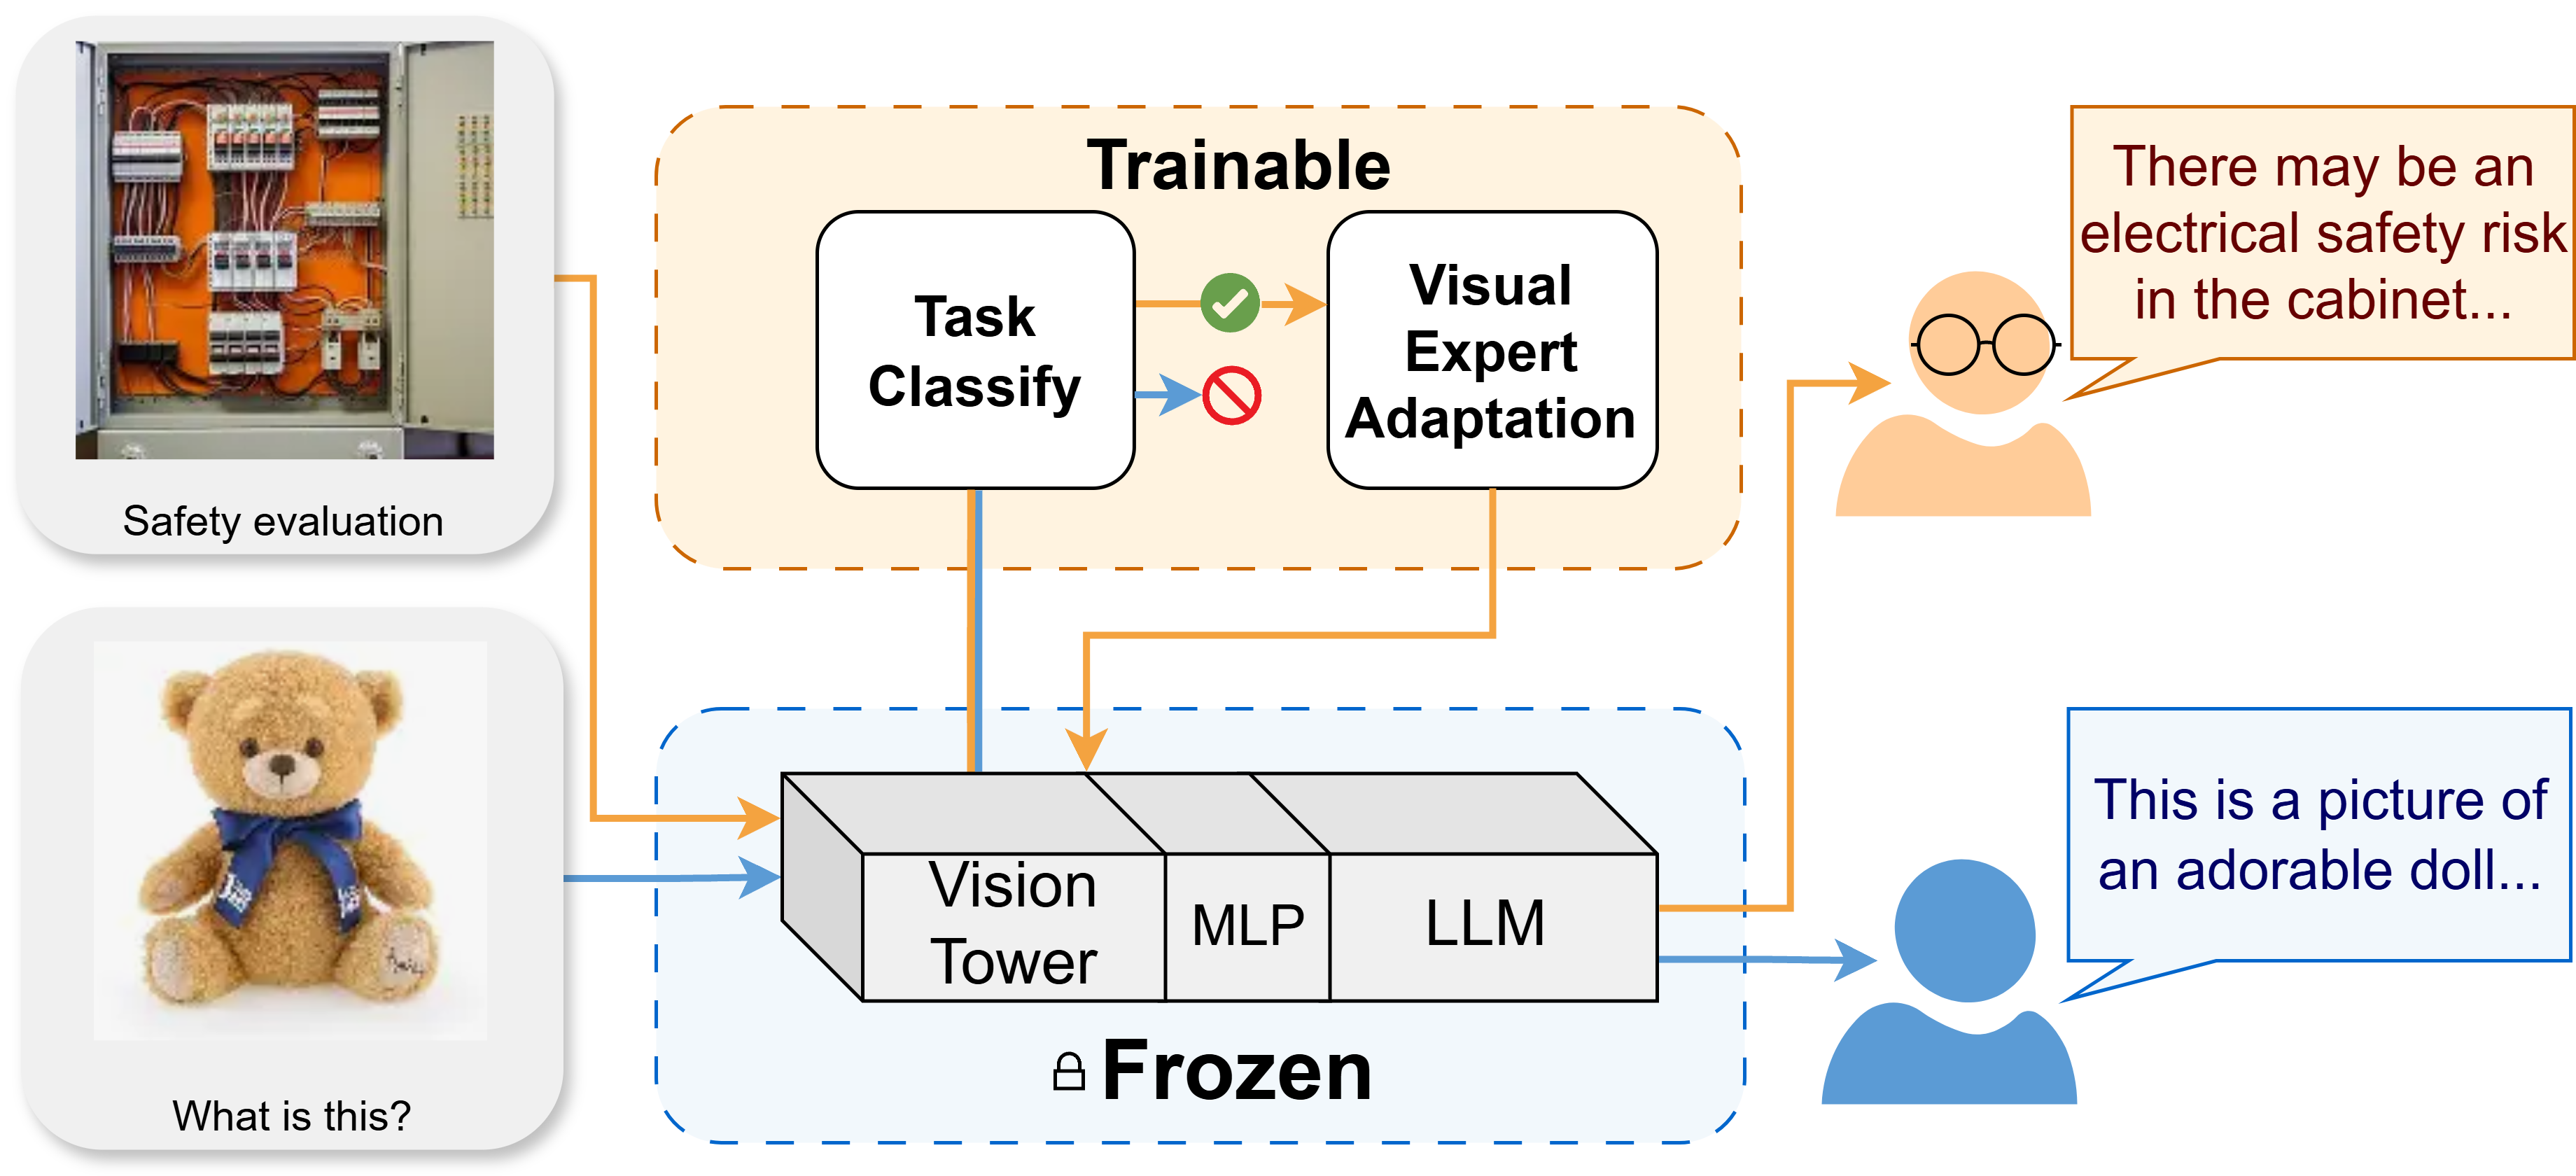
\includegraphics[width=0.9\linewidth]{正式版-抽象.png}
    \caption{所提出的即插即用适配框架整体架构。主干 VLM（包含视觉塔、MLP 和 LLM）被严格冻结。为了实现按需的知识注入且不发生灾难性遗忘，引入了一个外部可训练模块。通用查询（如识别玩具）直接绕过专业模块，确保对模型通用能力的零干扰；特定领域查询（如电气安全评估）则通过任务分类器激活专业视觉分支。最后，K-预算门（K-Budget Gate）动态控制专业表征注入回冻结主干的强度。}
    \label{fig:1}
\end{center}
}]

% 显示摘要和关键词区（不要动）
\IEEEdisplaynontitleabstractindextext
\IEEEpeerreviewmaketitle




% ==========================================
% 7. 正文部分：引言
% ==========================================
% ==========================================
% 7. 正文部分：引言
% ==========================================
\section{Introduction}

电力电气系统的安全稳定运行高度依赖对输电线路、变电站及配电设备的持续巡检与状态评估，而传统依赖人工经验的检测方式在效率、一致性和实时性方面已难以满足大规模运维需求\cite{rocha2025advances,liu2026review}。近年来，视觉-语言模型，尤其是视觉-语言大模型（Vision-Language Large Models, VLLMs），在图像理解、视觉问答和多模态指令跟随等任务上展现出较强能力\cite{zhang2024vision}。对于电力电气场景，这类模型有望统一支持缺陷识别、设备判读、巡检问答和结构化结果生成等多种图文联合任务，因而受到越来越多关注\cite{wang2024power,hao2025power}。

然而，电力电气领域的 VLLM 适配具有鲜明的专业约束。首先，该类任务专业性强、容错率低，许多设备类别和异常状态需要结合行业知识才能准确区分；其次，高质量专业多模态数据通常规模有限、标注成本高且类别分布不均衡\cite{lin2025defectgpt}；此外，实际部署还常受到边缘算力、训练预算和模型更新成本限制，单纯依赖大规模参数更新并不现实\cite{sharshar2025vision,jeon2026edgev}。因此，理想的领域适配方法不仅要增强专业能力，还应尽量保留原模型的通用视觉-语言能力，并控制训练与部署开销。

面向这一问题，最直接的方案是对预训练多模态模型进行全量微调，但该策略通常成本较高，并可能破坏预训练阶段获得的通用表征和指令跟随能力，导致灾难性遗忘\cite{zhai2023investigating,zhu2024model}。为此，LoRA、Adapter、Prompt Tuning 和 Prefix Tuning 等参数高效微调（PEFT）方法被广泛用于多模态模型适配\cite{hu2022lora,zhou2024empirical,wang2025parameter}。尽管这类方法在参数开销上更具优势，但多数仍通过统一调整共享主干内部表征来完成适配，难以显式控制专业知识何时介入、介入多少以及如何尽量避免对原有推理路径的扰动\cite{wu2026domain}。同时，围绕抗遗忘、动态专家和附加表征学习的相关研究也提供了有益启发，例如持续多模态调优中的稳定化专家机制与动态专家路由\cite{tuning83same,ge2025dynamic}，以及通过共享表征空间增强跨模态适配能力的 MMRL\cite{guo2025mmrl}。不过，这些方法大多面向持续学习场景、双塔视觉语言模型或主干可更新设定，而当前主流 VLLM 更常采用将视觉特征映射为 token 序列并与文本共同输入大语言模型的生成式架构\cite{radford2021learning,liu2023visual,bai2025qwen3}，因而现有方案难以直接满足电力电气场景中“主干冻结、按需注入、低干扰适配”的需求。

基于上述观察，本文提出一种面向电力电气专业场景的\textbf{外挂式冻结适配框架}。该方法在完全冻结原始多模态主干参数的前提下，引入轻量可训练专业模块，并借鉴共享表征学习思想，在生成式 VLLM 中实现视觉侧与语言侧的协同适配：在视觉编码阶段，通过条件门控按需激活专业视觉支路；在语言输入阶段，通过动态预算机制控制文本专家表示的注入强度。该框架无需直接修改基座模型参数，能够以插件化方式实现领域知识的稀疏调用，从而兼顾专业能力增强、通用能力保持以及后续多领域扩展性。

本文的主要贡献如下：
\begin{itemize}
    \item 提出一种面向电力电气专业场景的多模态冻结式外挂适配框架，在不更新原始 VLLM 主干参数的前提下实现领域增强；
    \item 构建适用于串行生成式 VLLM 的专业表示注入机制，并结合视觉条件门控与文本动态预算控制，实现专业知识的按需、低干扰介入；
    \item 在自建电力电气多模态测试集上的实验表明，所提方法能够显著提升专业任务表现，同时在通用任务上保持近零遗忘，验证了其在低成本专业化适配中的有效性。
\end{itemize}


\section{Related Work}

\subsection{多模态大模型的领域适配与参数高效微调}

随着多模态大模型的发展，如何在有限数据和有限算力条件下完成领域适配已成为重要研究问题\cite{zhou2024empirical}。全量微调能够较充分地拟合目标任务，但其训练成本高、参数更新范围大，不利于低成本部署。为降低适配开销，LoRA、Adapter、Prompt Tuning 和 Prefix Tuning 等 PEFT 方法被广泛用于语言模型及多模态模型\cite{hu2022lora,wang2025parameter}。已有研究也对多模态大模型中的 PEFT 效果进行了系统比较，表明其在效率与性能之间具有较好的折中\cite{zhou2024empirical}。在一些专业视觉语言任务中，动态 LoRA 路由等方法进一步尝试提升领域适配能力\cite{wu2026domain}。

然而，现有 PEFT 方法大多仍建立在“调整共享主干表征”的思路上，即使参数量较小，本质上仍会改变模型内部的表示分布与推理路径。对于电力电气这类高专业、强部署约束场景，这种统一式适配未必理想，因为专业知识并非所有输入都需要调用。本文因此选择在完全冻结主干的前提下，以外挂模块承载领域增量知识，并通过条件机制控制其是否介入及介入强度。

\subsection{抗遗忘适配与低干扰学习}

灾难性遗忘是多模态模型领域适配中的核心问题之一。已有研究指出，在多模态大模型微调过程中，模型原有的视觉知识、通用问答能力和指令跟随行为都可能因下游数据分布偏移而发生退化\cite{zhai2023investigating}。为缓解该问题，研究者提出了多种方案，例如更温和的微调策略、结构约束、选择性更新以及面向稳健适配的专门框架\cite{zhu2024model,li2026fine}；持续学习方向还探索了模型融合、重放和参数隔离等思路，以减轻新旧知识冲突\cite{gao2025enhanced}。在多模态持续指令调优场景中，稳定化混合专家和动态课程专家等方法也展现出一定的抗干扰能力\cite{tuning83same,ge2025dynamic}。

这些工作为稳健适配提供了重要参考，但多数仍默认需要直接或间接更新共享主干，再通过训练策略或结构约束减轻退化。相比之下，本文更强调一种结构层面的低干扰路径：尽可能不改变原始 VLLM 主干，而是将专业能力封装在可独立训练、可独立加载的外部模块中，以适应电力电气场景下对稳定性、可扩展性和更新成本的共同要求。

\subsection{动态路由、专家机制与共享表征学习}

为了提升模型容量利用率并缓解多任务表示冲突，动态路由与混合专家机制近年来被广泛研究。在大规模视觉语言模型中，MoE 结构已被用于增强模型容量和任务分工能力\cite{lin2026moe}。这类方法说明了条件计算在复杂多模态任务中的有效性，但其关注点通常是专家分配、容量扩展或任务解耦，而不是围绕专业知识在生成式 VLLM 中的按需、低干扰注入建立专门机制。

与本文关系更直接的是共享表征学习方向。CLIP 等双塔视觉语言模型通过对比学习获得可迁移的图文表示\cite{radford2021learning}，MMRL 则进一步通过共享的模态无关表征空间学习附加表示，以增强跨模态适配能力\cite{guo2025mmrl}。这一思想对本文具有重要启发：领域增量知识可以不直接写入冻结主干，而由独立的共享表示空间承载，再投影到不同模态侧发挥作用。然而，现有 MMRL 主要面向 CLIP 类双塔架构，其输出通常服务于图像特征与文本特征的对齐；而在生成式 VLLM 中，视觉信息需要先转换为 token 序列，再与文本嵌入共同输入大语言模型参与自回归生成\cite{liu2023visual,bai2025qwen3}。因此，本文并非直接复用双塔式方案，而是在冻结主干的生成式框架中，将共享表征思想扩展为视觉条件门控和文本动态预算相结合的协同注入机制，以满足电力电气专业场景中的低干扰适配需求。









\section{Methodology}

\begin{figure*}[t]
    \centering
    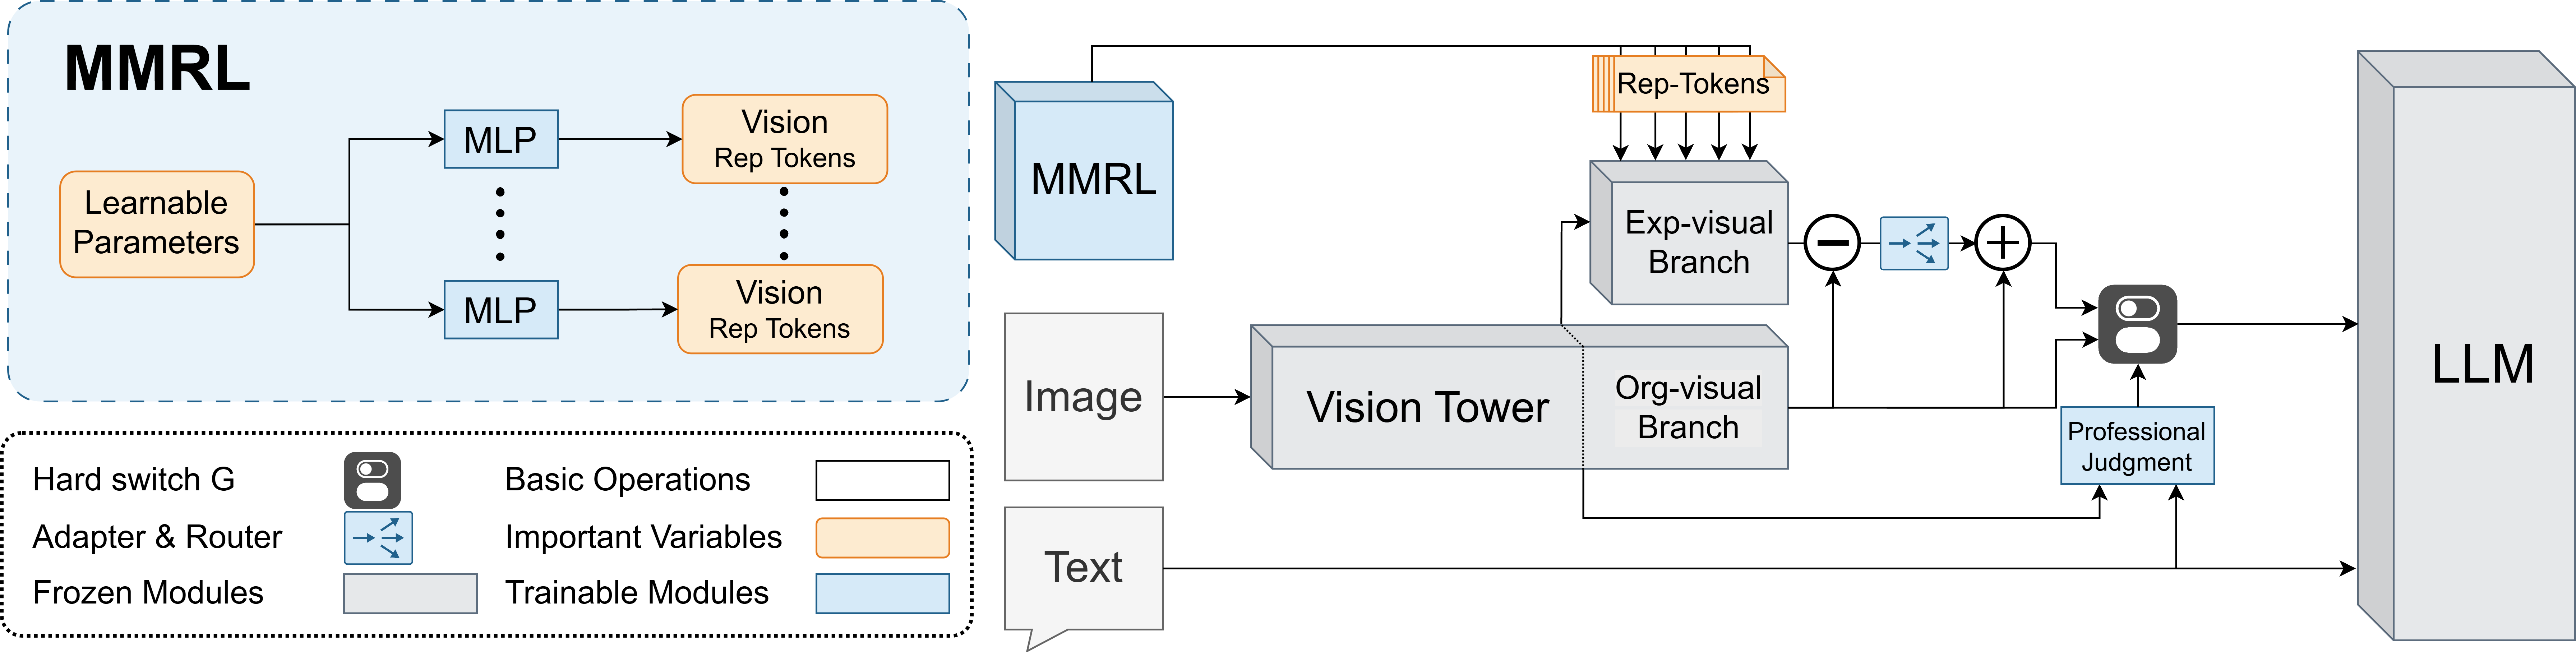
\includegraphics[width=\textwidth]{正式版-整体.png}
    \caption{本文所提出 MMRL 框架的整体结构示意图。MMRL 首先学习一组共享表示，并将其投影为不同视觉注入层所需的视觉代表 token；随后，任务分类器利用池化后的视觉状态与文本嵌入预测样本级增强需求，并通过 Hard-Concrete 门控控制增强分支是否生效；最后，视觉残差经由文本条件化的 router-adapter 模块进行选择性调制，再写回视觉表示。整个过程仅改变视觉编码阶段的表示，不改变语言模型侧的输入序列结构。}
    \label{fig:method_overview}
\end{figure*}

\subsection{Overview}
\label{sec:method_overview}

本文在 Qwen3-VL 框架上提出一种文本条件化的多模态表示路由机制（MMRL），旨在以较小结构改动增强视觉表征，并保持语言模型输入与解码过程的稳定性。整体方法可分为三个部分：\textbf{(1) MMRL 视觉代表 token 生成}，构建可学习共享表示空间，并为不同视觉注入层生成层特定的代表 token；\textbf{(2) 文本条件任务门控}，基于图像全局特征与文本全局特征预测样本级激活信号，用于判断当前输入是否需要启用视觉增强路径；\textbf{(3) 视觉增强与残差路由}，在视觉编码器的若干指定层中插入或更新视觉代表 token，并通过门控残差与 adapter router 对原始视觉特征进行条件调制。

与直接拼接额外特征或修改语言侧 token 序列不同，本文方法将增强集中在视觉编码阶段。文本嵌入仅作为任务判断和路由选择的条件上下文，不作为被写入或改写的对象。因此，增强后的视觉 token 在被写回多模态输入嵌入之前已经完成调制，而后续语言模型仍接收标准的多模态输入结构。如图~\ref{fig:method_overview} 所示，MMRL 在保留原始主干稳定性的同时，为视觉表示引入样本相关的条件增强能力。

这一设计也来自方法迭代中的经验观察。多轮实验表明，语言侧显式改写对最终指标的提升有限；同时，在自回归解码过程中动态改变语言侧可见位置会影响注意力结构、位置状态与 KV cache 的一致性，增加推理实现的不稳定性。因此，本文选择不修改语言模型侧输入序列和注意力结构，而是将可学习增强限制在视觉编码器内部，以兼顾性能收益、推理效率与系统稳定性。


\subsection{MMRL表征token生成}
\label{sec:mmrl_token_generation}

为向视觉编码器提供可学习的全局语义先验，本文首先定义一个共享表示空间
\begin{equation}
\mathbf{R}\in\mathbb{R}^{L\times d_s},
\end{equation}
其中，$L$ 表示代表 token 的数量，$d_s$ 表示共享表示维度。$\mathbf{R}$ 可视为一组全局可学习的表征基元，其参数在训练过程中端到端优化。

对于第 $l$ 个视觉注入层，本文使用层特定的轻量投影函数将共享表示映射到视觉特征空间：
\begin{equation}
\mathbf{R}^{(l)}_{v}=f^{(l)}_{v}(\mathbf{R}),
\end{equation}
其中，$f^{(l)}_{v}(\cdot)$ 表示对应层的线性投影网络，$\mathbf{R}^{(l)}_{v}\in\mathbb{R}^{L\times d_v}$，$d_v$ 为视觉编码器隐藏维度。由于不同注入层处于视觉编码器的不同语义深度，层特定投影使同一共享表示能够适配不同层级的视觉特征分布。

在推理阶段，$\mathbf{R}$ 及其投影结果与具体样本无关，因此视觉代表 token 可以在首次计算后缓存复用，从而避免重复投影开销。该设计只引入少量可学习参数，却能够为后续视觉增强分支提供稳定的全局先验。


\subsection{任务分类器}
\label{sec:task_classifier}

为判断当前样本是否需要启用视觉增强分支，本文设计了一个轻量任务分类器。其核心包括两个步骤：首先利用\textbf{基于可学习查询向量的注意力池化}提取视觉与文本的全局摘要；随后基于联合摘要预测任务相关分数，并通过 \textbf{Hard-Concrete} 松弛生成近似二值门控。\cite{louizos2017learning}

设某一模态的输入序列表示为
\begin{equation}
\mathbf{X}=[\mathbf{x}_1,\mathbf{x}_2,\ldots,\mathbf{x}_S]\in\mathbb{R}^{S\times d}.
\end{equation}
不同于固定平均池化，本文引入一个可学习查询向量 $\mathbf{q}\in\mathbb{R}^{d}$，并分别对查询与输入 token 做线性投影：
\begin{equation}
\hat{\mathbf{q}}=\mathbf{W}_q\mathbf{q},\qquad
\hat{\mathbf{x}}_i=\mathbf{W}_e\mathbf{x}_i.
\end{equation}
随后通过缩放点积注意力计算每个 token 的聚合权重
\begin{equation}
a_i=\frac{\exp\left(\hat{\mathbf{q}}^\top \hat{\mathbf{x}}_i/\sqrt{d_p}\right)}
{\sum_{j=1}^{S}\exp\left(\hat{\mathbf{q}}^\top \hat{\mathbf{x}}_j/\sqrt{d_p}\right)}.
\end{equation}
若存在有效位置掩码，则仅在合法位置上归一化。最终得到该模态的全局表示
\begin{equation}
\mathbf{g}=\mathrm{LN}\left(\sum_{i=1}^{S} a_i \mathbf{x}_i\right),
\end{equation}
其中 $\mathrm{LN}(\cdot)$ 表示 LayerNorm。该池化过程分别作用于视觉 token 序列与文本 embedding 序列，从而得到视觉全局表示 $\mathbf{g}_v$ 和文本全局表示 $\mathbf{g}_t$。这里的文本全局表示仅作为条件上下文参与任务判断，不改变原始文本嵌入本身。

在此基础上，任务分类器将两种模态的摘要进行融合，并输出一个标量分数
\begin{equation}
\alpha=\mathrm{MLP}\big([\mathbf{g}_v;\mathbf{g}_t]\big),
\end{equation}
其中 $\alpha\in\mathbb{R}$ 表示当前样本对视觉增强分支的需求强度。为获得可训练的稀疏门控，本文进一步采用 Hard-Concrete 松弛。训练阶段，首先采样
\begin{equation}
u\sim \mathrm{Uniform}(0,1),\qquad
\epsilon=\log u-\log(1-u),
\end{equation}
并构造连续松弛变量
\begin{equation}
\tilde{g}=\sigma\left(\frac{\alpha+\epsilon}{\tau}\right),
\end{equation}
其中 $\sigma(\cdot)$ 为 Sigmoid 函数，$\tau$ 为温度系数。随后，对其进行区间拉伸与截断：
\begin{equation}
G=\min\!\left(1,\max\!\left(0,\tilde{g}(\zeta-\gamma)+\gamma\right)\right),
\end{equation}
其中 $\gamma<0,\zeta>1$ 为超参数，因而 $G\in[0,1]$ 可被视为近似二值的软门控。推理阶段去除随机噪声，并可进一步按照阈值将其离散化为硬门控结果。

因此，任务分类器的输出并非简单的类别预测，而是一个由视觉--文本联合上下文驱动的门控信号，用于控制后续视觉增强残差是否参与最终特征融合。

\begin{figure*}[t]
    \centering
    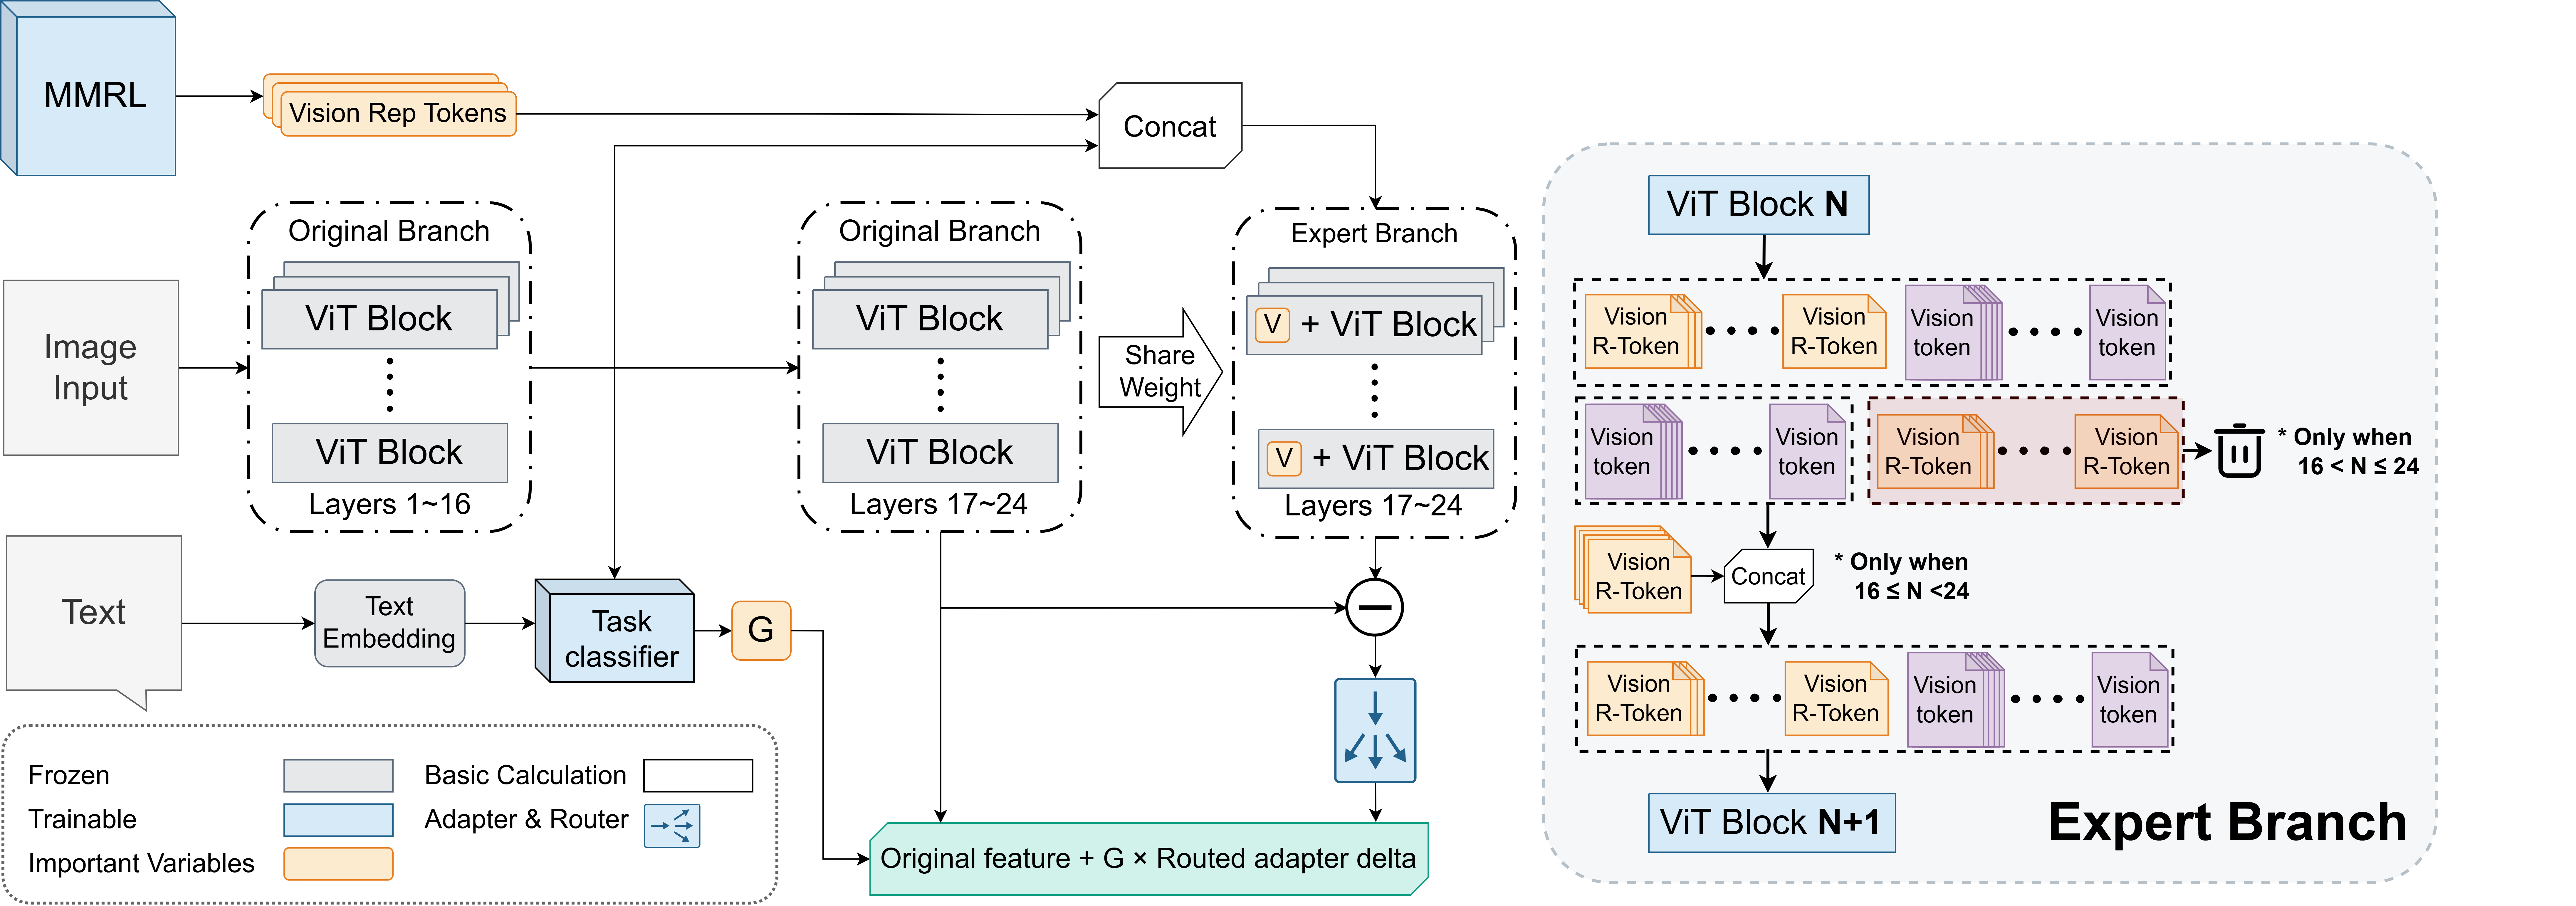
\includegraphics[width=\textwidth]{正式版-视觉部分.png}
    \caption{
    任务分类器与视觉增强支路的整体框架。MMRL 首先生成视觉代表 token，并在视觉编码器的指定层中插入或更新，以形成增强分支。任务分类器对中间视觉状态与文本嵌入进行注意力池化和特征融合，输出任务相关分数 $\alpha$，再经 Hard-Concrete 映射为门控变量 $G$。在此基础上，模型对原始分支和增强分支的差异进行门控与残差路由，从而获得任务自适应的视觉表示。
    }
    \label{fig:task_classifier_visual_branch}
\end{figure*}


\subsection{视觉支路}
\label{sec:visual_branch}

在视觉编码阶段，本文在原始视觉主干之外构建一条由代表 token 驱动的增强分支。设视觉编码器共有若干层，记第 $l$ 层输入的视觉 token 序列为
\begin{equation}
\mathbf{H}^{(l)}\in\mathbb{R}^{N_l\times d_v},
\end{equation}
其中 $N_l$ 为该层 token 数量，$d_v$ 为视觉特征维度。令 $\mathcal{I}=\{l_1,l_2,\dots,l_M\}$ 表示预先选定的注入层索引集合，对应的视觉代表 token 由前述共享表示模块生成，即
\begin{equation}
\mathbf{R}_v^{(l_m)}\in\mathbb{R}^{L\times d_v}, \qquad l_m\in\mathcal{I}.
\end{equation}

对于原始分支，视觉特征按照标准 Transformer block 正常传播：
\begin{equation}
\mathbf{H}_{\mathrm{org}}^{(l+1)}=\mathcal{F}^{(l)}\!\left(\mathbf{H}_{\mathrm{org}}^{(l)}\right),
\end{equation}
其中 $\mathcal{F}^{(l)}(\cdot)$ 表示第 $l$ 个视觉块。与此同时，增强分支在指定层引入视觉代表 token，并与原始分支共享相同的视觉块参数。对于第一次注入层 $l_1$，采用前缀拼接方式：
\begin{equation}
\mathbf{H}_{\mathrm{exp}}^{(l_1)}=
\left[
\mathbf{R}_v^{(l_1)};\,
\mathbf{H}_{\mathrm{org}}^{(l_1)}
\right].
\end{equation}
这样，代表 token 将与原始视觉 token 一同参与后续自注意力计算。

为避免序列长度随着注入层数持续增长，在后续注入层 $l_m\,(m>1)$ 中，仅对前部代表 token 槽位进行更新，而不再重复扩展序列。记增强分支在该层进入 block 前的前缀部分为 $\mathbf{H}_{\mathrm{exp},1:L}^{(l_m)}$，则可写为
\begin{equation}
\mathbf{H}_{\mathrm{exp},1:L}^{(l_m)}
\leftarrow
\Psi\!\left(
\mathbf{H}_{\mathrm{exp},1:L}^{(l_m)},
\mathbf{R}_v^{(l_m)}
\right),
\end{equation}
其中 $\Psi(\cdot)$ 表示前缀更新操作。在本文实现中，该操作可采用替换或加性更新两种形式，即
\begin{equation}
\Psi_{\mathrm{rep}}(\mathbf{A},\mathbf{B})=\mathbf{B},
\qquad
\Psi_{\mathrm{add}}(\mathbf{A},\mathbf{B})=\mathbf{A}+\mathbf{B}.
\end{equation}
随后增强分支继续经过共享参数的视觉块：
\begin{equation}
\mathbf{H}_{\mathrm{exp}}^{(l+1)}=\mathcal{F}^{(l)}\!\left(\mathbf{H}_{\mathrm{exp}}^{(l)}\right).
\end{equation}

\begin{figure*}[t]
    \centering
    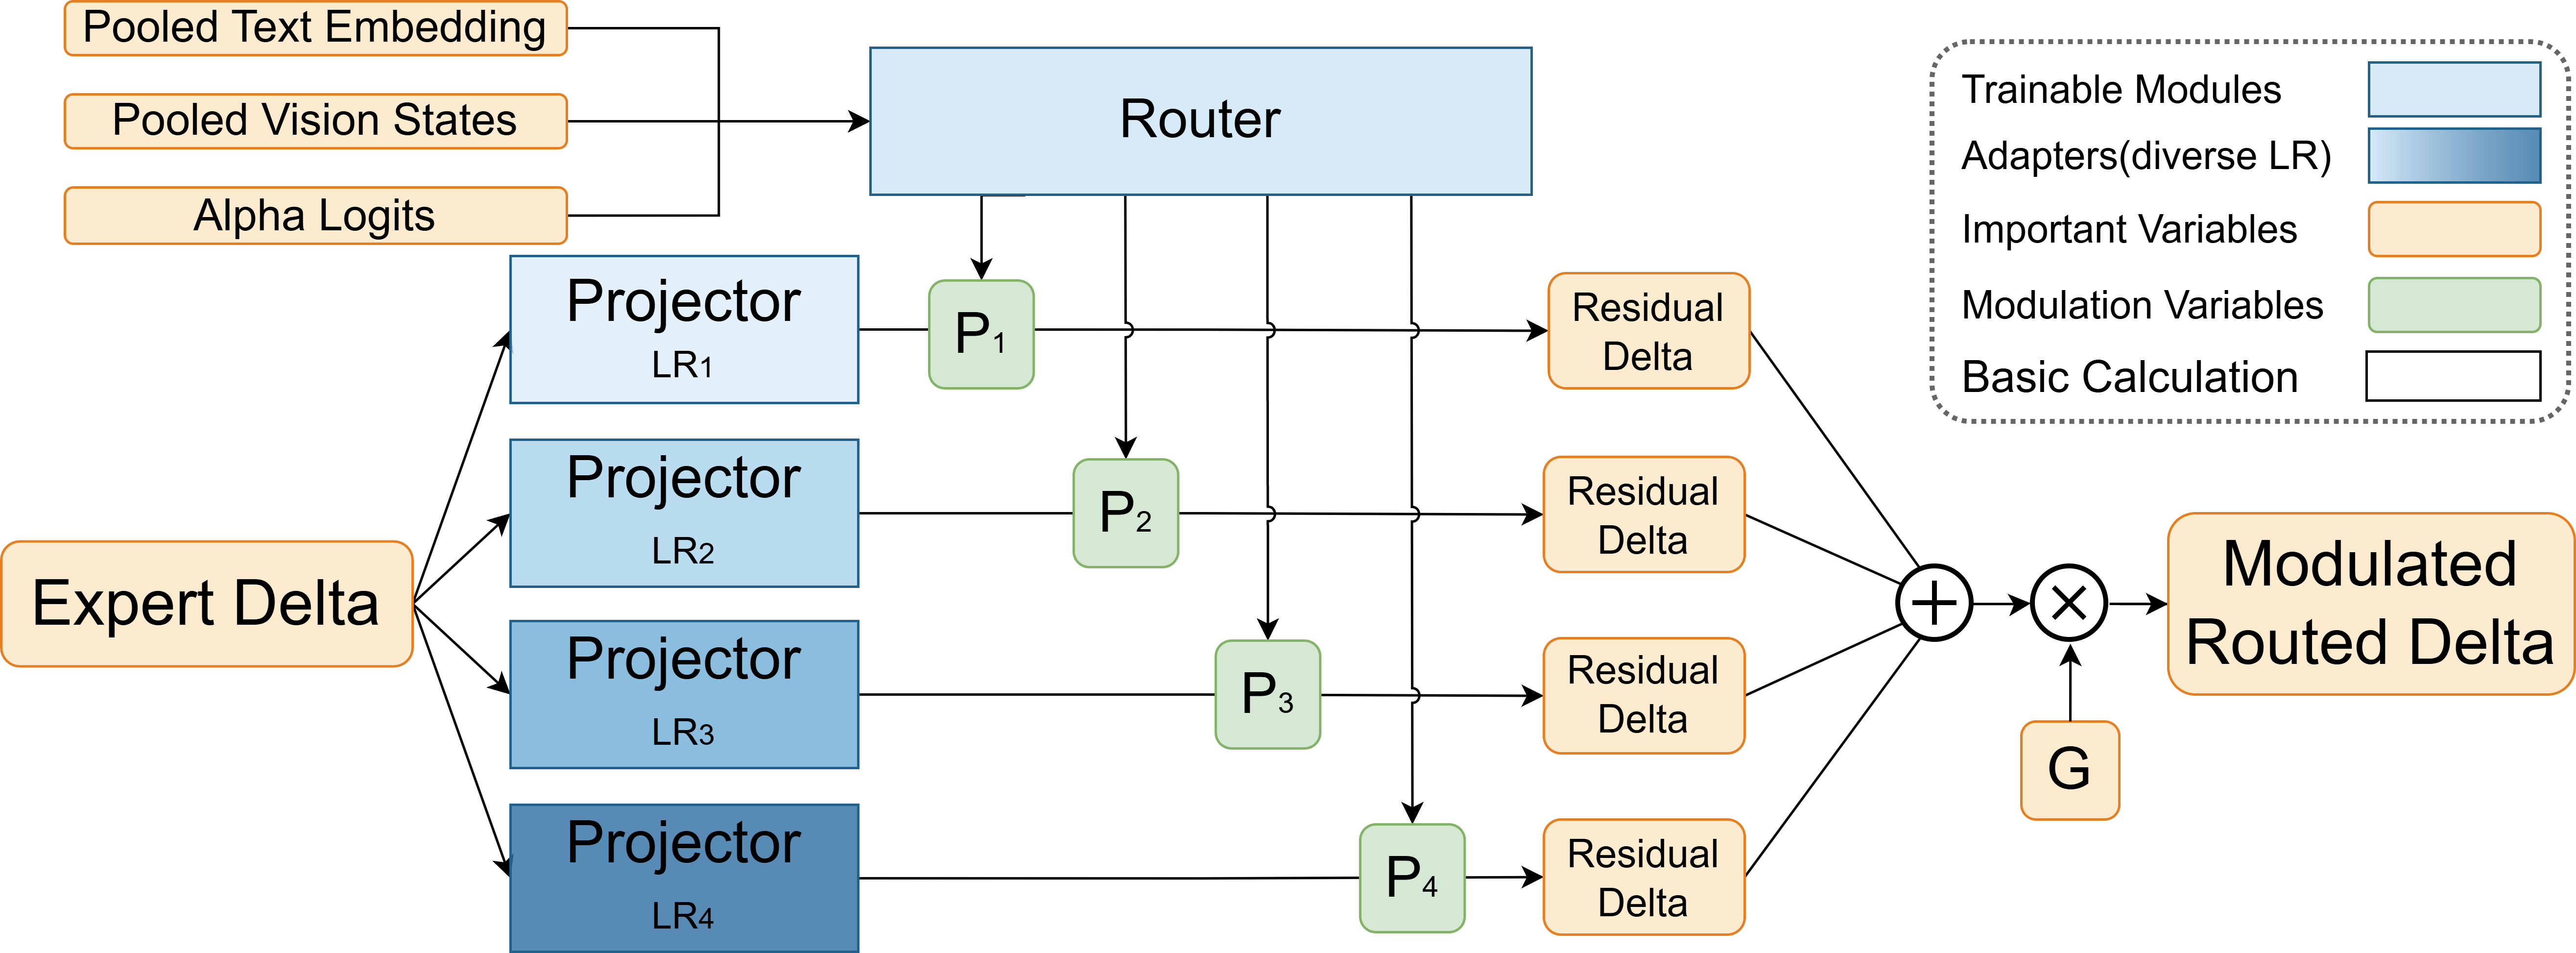
\includegraphics[width=0.92\linewidth]{正式版-路由器.png}
    \caption{视觉 residual adapter router 设计示意图。模型首先利用池化视觉表示、池化文本表示及 expertise score 生成各视觉残差适配器的路由权重；随后，各残差适配器分别对门控后的视觉残差进行变换，并经加权求和后写回原始视觉状态，得到最终视觉隐藏表示。该模块是后续路由均衡、熵约束、共模抑制、有效残差约束、原型锚定与适配器多样性约束的共同作用对象。}
    \label{fig:shared_router_adapter}
\end{figure*}

在最后一个注入层之后，增强分支前部的代表 token 被移除，以恢复与原始分支一致的 patch-token 对齐形式。记去除代表 token 后的增强分支输出为 $\hat{\mathbf{H}}_{\mathrm{exp}}$，则两条分支之间的视觉残差可定义为
\begin{equation}
\mathbf{\Delta}=\hat{\mathbf{H}}_{\mathrm{exp}}-\mathbf{H}_{\mathrm{org}},
\end{equation}
其中 $\mathbf{H}_{\mathrm{org}}$ 表示对应层级下原始分支的输出。进一步地，由上一小节得到的任务相关门控 $G\in[0,1]$ 用于控制该残差增量的激活程度。将 $G$ 广播到对应图像的全部视觉 token 后，可得
\begin{equation}
\mathbf{\Delta}_g = G \odot \mathbf{\Delta},
\end{equation}
其中 $\odot$ 表示逐元素乘法。由此，当 $G=0$ 时，增强分支产生的残差被完全抑制；当 $G$ 接近 $1$ 时，该残差则被基本完整地保留下来，从而对原始视觉表征形成有效补充。

为提升视觉残差调制的表达能力，本文不直接将 $\mathbf{\Delta}_g$ 加回主干特征，而是引入多个残差适配器进行条件路由。该设计可视为一种用于视觉残差的轻量 mixture-of-experts 结构：不同适配器负责学习不同类型的视觉残差变换，路由器则根据当前图像、文本上下文以及增强需求强度，为每个样本选择合适的残差组合。\cite{shazeer2017outrageously}\cite{houlsby2019parameter}

设共有 $K$ 个视觉适配器 $\{\mathcal{A}_k\}_{k=1}^K$。路由器以视觉全局表示 $\mathbf{g}_v$、文本全局表示 $\mathbf{g}_t$ 以及门控概率 $\sigma(\alpha)$ 为输入，生成适配器权重
\begin{equation}
\boldsymbol{\pi}
=
\mathrm{Softmax}\left(
f_r\big([\mathbf{g}_v;\mathbf{g}_t;\sigma(\alpha)]\big)
\right),
\end{equation}
其中 $\boldsymbol{\pi}=[\pi_1,\ldots,\pi_K]$，满足
\begin{equation}
\sum_{k=1}^{K}\pi_k=1,\qquad \pi_k\ge 0.
\end{equation}
在实现上，路由器分别对 $\mathbf{g}_v$ 与 $\mathbf{g}_t$ 做非线性投影，再与 $\sigma(\alpha)$ 拼接后输出 $K$ 维 logits。由于 $\sigma(\alpha)$ 表示样本对增强分支的整体需求，路由器不仅能够感知“是否需要增强”，还能够进一步决定“应当以哪种专家残差进行增强”。这一区分对于防止单一残差模式主导训练尤为重要；若直接使用一个共享适配器，模型很容易将训练集中的局部偏差编码进唯一残差通道，从而导致泛化能力下降。

每个适配器采用瓶颈式残差变换：
\begin{equation}
\mathcal{A}_k(\mathbf{x})
=
\mathbf{W}^{(k)}_{\mathrm{up}}
\phi\!\left(
\mathbf{W}^{(k)}_{\mathrm{down}}\mathbf{x}
\right),
\end{equation}
其中 $\phi(\cdot)$ 表示非线性激活函数。本文将适配器最后一层初始化为零，使训练初期的增强路径接近关闭状态，避免在优化早期破坏预训练视觉主干。最终的视觉增强项表示为
\begin{equation}
\mathbf{\Delta}^{*}
=
\sum_{k=1}^{K}\pi_k\,\mathcal{A}_k(\mathbf{\Delta}_g),
\end{equation}
并得到视觉支路的最终输出
\begin{equation}
\mathbf{H}_{\mathrm{out}}
=
\mathbf{H}_{\mathrm{org}}
+
\mathbf{\Delta}^{*}.
\end{equation}

上述 router-adapter 结构不仅增加了视觉残差的表达能力，也是抑制过拟合的关键设计。视觉代表 token 会产生较强的可学习残差信号；若所有样本共享同一个残差变换，该信号容易退化为对训练集共性偏差的记忆。本文因此将残差调制分解为多个专家适配器，并通过样本相关路由进行组合，使不同类型的视觉增强由不同专家承担。后续训练目标将进一步约束路由分布与专家输出，以避免路由塌缩和专家冗余。\cite{fedus2022switch}

基于 Qwen3-VL 的 DeepStack 多层视觉特征路径，本文进一步将 MMRL 产生的门控视觉残差注入对应中间层特征，使最终视觉输出与 deepstack 特征同时受条件增强机制调制。对于被选入 deepstack 的视觉层 $l$，记去除代表 token 后的局部增强分支输出为 $\hat{\mathbf{H}}_{\mathrm{exp}}^{(l)}$，原始分支输出为 $\mathbf{H}_{\mathrm{org}}^{(l)}$，则该层的 deepstack 输入特征定义为
\begin{equation}
\mathbf{D}^{(l)}
=
\mathbf{H}_{\mathrm{org}}^{(l)}
+
\lambda_{\mathrm{ds}}\,
G\odot
\left(
\hat{\mathbf{H}}_{\mathrm{exp}}^{(l)}
-
\mathbf{H}_{\mathrm{org}}^{(l)}
\right),
\end{equation}
其中 $\lambda_{\mathrm{ds}}$ 为 deepstack 残差缩放系数。这样，最终视觉输出与中间层视觉特征都能够接收由同一门控信号控制的 MMRL 增强；深层语言模型不仅看到最终合并后的视觉 token，也能够通过 deepstack 路径获得多层次的条件增强视觉信息。

因此，视觉支路并非直接以代表 token 替代原始视觉特征，而是在保持原始主干稳定传播的基础上，利用代表 token 构造增强分支，并结合任务门控与文本条件化残差路由实现样本相关的视觉调制。增强完成后，模型仅将调制后的视觉表示交回多模态主干，语言模型侧的输入组织方式保持不变。




















\subsection{Training Objective}
\label{sec:training_objective}

本文采用四阶段训练策略，其基本原则是“先学习任务判别与门控，再学习共享表征及其双分支注入”。这一设计的动机在于：任务分类器主要依赖视觉/文本的全局嵌入统计，因此在前两阶段可以利用由多模态样本经模板组合与规则清洗得到的辅助文本视图进行稳健预训练；而 MMRL 表征空间、视觉增强分支和文本注入分支所学习的是更细粒度的领域知识结构，因此后续阶段仅使用高质量专业语料，并建立在门控变量 $G$ 已基本收敛的前提下进行优化。换言之，Stage 3--4 中的知识注入是在近乎离散的可靠门控约束下完成的，这也是本文采用多阶段训练而非直接端到端联合优化的关键原因。

\paragraph{Stage 1: task classifier pretraining.}
第一阶段仅训练池化模块与任务分类器，使模型先获得稳定的样本级任务可分性。记任务分类器输出的 expertise score 为 $\alpha\in\mathbb{R}$，监督标签为 $y\in\{0,1\}$，则该阶段目标定义为
\begin{equation}
\mathcal{L}_{\mathrm{S1}}=\mathcal{L}_{\mathrm{cls}}^{(1)}(\alpha,y).
\end{equation}
在实现中，$\mathcal{L}_{\mathrm{cls}}^{(1)}$ 采用 focal binary cross-entropy，以减轻类别不均衡对早期判别边界学习的不利影响。此时 Hard-Concrete 门控尚不直接参与训练，其作用仅限于为下一阶段提供可初始化的判别分数。

\paragraph{Stage 2: gate fitting.}
第二阶段在保留分类监督的同时，进一步显式优化门控模块。记由 Hard-Concrete 变换得到的连续门控输出为
\begin{equation}
G=\mathrm{HC}(\alpha),
\end{equation}
则该阶段损失写为
\begin{equation}
\mathcal{L}_{\mathrm{S2}}
=
\mathcal{L}_{\mathrm{cls}}^{(2)}(\alpha,y)
+
\lambda_{g}\,\mathcal{L}_{\mathrm{gate}}(G,y),
\end{equation}
其中 $\mathcal{L}_{\mathrm{cls}}^{(2)}$ 在实现中采用 standard BCE with logits，而
\begin{equation}
\mathcal{L}_{\mathrm{gate}}(G,y)=\|G-y\|_2^2 .
\end{equation}
经过 Stage 1--2 之后，$\alpha$ 与 $G$ 通常已经形成清晰的两极分布，亦即大多数样本的门控值会稳定在接近 $0$ 或 $1$ 的区域。因此，在后续训练中，虽然实现上仍保留 Hard-Concrete 的连续形式以维持计算图一致性，但从方法语义上可将 $G$ 近似视为离散门控变量。该性质对于本文尤为重要，因为无论视觉增强支路还是文本注入支路，都是在这一近似硬门控约束下被选择性激活的。

\paragraph{Stage 3--4: full optimization of MMRL.}
第三、四阶段开始优化完整的 MMRL 主体，包括共享表示空间、视觉残差适配器、文本残差适配器以及两侧的路由器。设训练样本为 $(\mathbf{I},\mathbf{x},\mathbf{y})$，其中 $\mathbf{I}$ 表示输入图像，$\mathbf{x}$ 表示输入文本，$\mathbf{y}$ 表示目标输出序列，则主任务损失采用标准自回归生成交叉熵：
\begin{equation}
\mathcal{L}_{\mathrm{CE}}
=
-\sum_{t=1}^{T}
\log p\!\left(y_t \mid y_{<t},\mathbf{x},\mathbf{I}\right).
\end{equation}

然而，仅依赖 $\mathcal{L}_{\mathrm{CE}}$ 往往不足以稳定训练基于 router-adapter 的双分支结构。一方面，路由概率容易塌缩到少数适配器；另一方面，不同样本的增强残差可能退化为相似的共模偏移，从而削弱条件增强的样本特异性。因此，本文在 Stage 3--4 中进一步引入视觉侧和文本侧的结构正则。

\paragraph{Visual-side regularization.}
设一个 mini-batch 中共有 $N_v$ 个图像实例，视觉残差适配器数目为 $K_v$。对于第 $i$ 个图像，其视觉路由器输出的概率向量记为
\begin{equation}
\boldsymbol{\pi}^{(v)}_i
=
\left[\pi^{(v)}_{i1},\pi^{(v)}_{i2},\ldots,\pi^{(v)}_{iK_v}\right],
\qquad
\sum_{k=1}^{K_v}\pi^{(v)}_{ik}=1.
\end{equation}
首先，为避免所有样本集中使用同一个适配器，定义 batch 级平均使用率
\begin{equation}
\bar{\pi}^{(v)}_{k}
=
\frac{1}{N_v}\sum_{i=1}^{N_v}\pi^{(v)}_{ik},
\end{equation}
并将其与均匀分布进行约束，从而得到视觉使用均衡损失
\begin{equation}
\mathcal{L}_{\mathrm{v\_bal}}
=
\sum_{k=1}^{K_v}
\bar{\pi}^{(v)}_{k}
\left(
\log \bar{\pi}^{(v)}_{k}
-
\log \frac{1}{K_v}
\right).
\end{equation}

其次，为避免单一样本的路由分布过于尖锐，记第 $i$ 个样本的路由熵为
\begin{equation}
\mathcal{H}^{(v)}_i
=
-
\sum_{k=1}^{K_v}
\pi^{(v)}_{ik}\log \pi^{(v)}_{ik},
\end{equation}
并给定目标熵阈值 $h_v$，则样本级熵正则写为
\begin{equation}
\mathcal{L}_{\mathrm{v\_ent}}
=
\frac{1}{N_v}
\sum_{i=1}^{N_v}
\max\!\left(0,\, h_v-\mathcal{H}^{(v)}_i\right).
\end{equation}

进一步地，设经过门控与路由后的最终视觉增强残差为 $\mathbf{\Delta}^{*}_i$，并记其池化表示为
\begin{equation}
\mathbf{z}^{(v)}_i=\mathrm{Pool}\!\left(\mathbf{\Delta}^{*}_i\right).
\end{equation}
若不同图像的增强方向过于一致，则说明模型退化为对所有样本施加近似相同的偏移。为抑制这种现象，定义视觉共模比例
\begin{equation}
r_v
=
\frac{
\left\|
\frac{1}{N_v}\sum_{i=1}^{N_v}\mathbf{z}^{(v)}_i
\right\|_2
}{
\frac{1}{N_v}\sum_{i=1}^{N_v}\|\mathbf{z}^{(v)}_i\|_2+\varepsilon
},
\end{equation}
并设目标上界为 $c_v$，则视觉共模抑制项为
\begin{equation}
\mathcal{L}_{\mathrm{v\_com}}
=
\max(0,\, r_v-c_v).
\end{equation}

\paragraph{Text-side regularization.}
类似地，设一个 batch 中共有 $N_t$ 个文本样本，文本残差适配器数目为 $K_t$。对于第 $b$ 个样本，其文本路由概率向量记为
\begin{equation}
\boldsymbol{\rho}^{(t)}_b
=
\left[\rho^{(t)}_{b1},\rho^{(t)}_{b2},\ldots,\rho^{(t)}_{bK_t}\right],
\qquad
\sum_{k=1}^{K_t}\rho^{(t)}_{bk}=1.
\end{equation}
文本适配器的使用均衡项定义为
\begin{equation}
\bar{\rho}^{(t)}_{k}
=
\frac{1}{N_t}\sum_{b=1}^{N_t}\rho^{(t)}_{bk},
\qquad
\mathcal{L}_{\mathrm{t\_bal}}
=
\sum_{k=1}^{K_t}
\left(
\bar{\rho}^{(t)}_{k}-\frac{1}{K_t}
\right)^2.
\end{equation}

同理，文本路由熵记为
\begin{equation}
\mathcal{H}^{(t)}_b
=
-
\sum_{k=1}^{K_t}
\rho^{(t)}_{bk}\log \rho^{(t)}_{bk},
\end{equation}
则对应的熵正则为
\begin{equation}
\mathcal{L}_{\mathrm{t\_ent}}
=
\frac{1}{N_t}
\sum_{b=1}^{N_t}
\max\!\left(0,\, h_t-\mathcal{H}^{(t)}_b\right).
\end{equation}

对于文本注入分支，记第 $b$ 个样本在所有有效占位符位置上的注入增量平均值为 $\mathbf{z}^{(t)}_b$，则文本共模比例可定义为
\begin{equation}
r_t
=
\frac{
\left\|
\frac{1}{N_t}\sum_{b=1}^{N_t}\mathbf{z}^{(t)}_b
\right\|_2
}{
\frac{1}{N_t}\sum_{b=1}^{N_t}\|\mathbf{z}^{(t)}_b\|_2+\varepsilon
},
\end{equation}
并得到文本共模抑制项
\begin{equation}
\mathcal{L}_{\mathrm{t\_com}}
=
\max(0,\, r_t-c_t),
\end{equation}
其中 $c_t$ 为文本侧允许的最大共模比例。该项用于约束不同样本的文本注入向量不要过度塌缩到同一方向，从而保留由视觉上下文和门控状态共同决定的样本差异性。

\paragraph{Overall loss for Stage 3--4.}
综合以上各项，Stage 3--4 的总损失可统一写为
\begin{align}
\mathcal{L}_{\mathrm{S}3/\mathrm{S}4}
=
&\;
\lambda_{\mathrm{ce}}\mathcal{L}_{\mathrm{CE}}
+\lambda_{vb}\mathcal{L}_{\mathrm{v\_bal}}
+\lambda_{ve}\mathcal{L}_{\mathrm{v\_ent}}
+\lambda_{vc}\mathcal{L}_{\mathrm{v\_com}}
\nonumber\\
&\;
+\lambda_{tb}\mathcal{L}_{\mathrm{t\_bal}}
+\lambda_{te}\mathcal{L}_{\mathrm{t\_ent}}
+\lambda_{tc}\mathcal{L}_{\mathrm{t\_com}}.
\label{eq:full_loss}
\end{align}
其中，各 $\lambda$ 为对应损失项的权重系数。与前两个阶段不同，此时优化的重点不再是学习门控边界本身，而是在门控已基本可靠的条件下，学习共享表征空间如何以视觉增强和文本注入两种方式安全地写入领域知识。也正因此，Stage 3--4 对训练语料质量显著更敏感：若在此阶段引入噪声较大的样本，则错误知识可能被 MMRL 表征空间及其双分支适配器显式吸收，进而削弱专业任务上的泛化能力。







% 本论文设计了以下几种实验：
% 1、与 LoRA(rank 8/16/32)、基座模型、更大开源模型、闭源模型对比
% 2、ABCD 四种文本注入策略对比
% 3、500 个通用任务样本上的通用性保持实验
% 专业支路启动率
% 与原模型输出 KL 散度
% 首 token top-1 相同率
% top-20 相似度
% 4、关键模块拆解消融
% 拆掉视觉门控使其永久附着
% 拆掉文本门控使得20个全开
% 把MMRL换成40个可学习参数
% 让视觉支路不可学习
% ###以下放到附录去
% 5、推理速度对比，参数量对比拉表
% 6、未学习过的场景识别
% 7、注意力热图
\section{Experiment}

\subsection{Experimental Setup}

\subsubsection{Domain Dataset Construction}

由于电力电气领域缺乏可直接用于多模态指令学习的公开数据，本文基于公开视觉资源构建领域训练集与测试题集，用于验证模型在专业场景中的适配能力。具体而言，我们从 14 个公开电力电气相关目标检测数据集中收集原始图像与标注，并对原始样本进行统一整理、低质量样本剔除和人工筛选，重点保证图像清晰度、标注可靠性、目标可辨识性、场景语义完整性和类别多样性。

筛选后的数据主要覆盖两类专业任务：
\begin{itemize}
    \item \textbf{设备与部件识别}：包括绝缘子、间隔棒、防振锤、断路器、互感器、变压器、隔离开关等典型电力设备与部件；
    \item \textbf{缺陷与异常检测}：包括异物悬挂、鸟巢、部件缺失、松动、破损、状态异常及植被侵扰等典型异常场景。
\end{itemize}

在训练数据构建阶段，本文使用 \texttt{Gemma 3 27b it} 作为辅助数据生成模型，将传统目标检测样本转换为 LLAVA 格式的多模态指令数据。生成过程中显式注入检测标签、类别名称、目标数量及场景信息，并根据任务类型与样本复杂度采用不同提示模板，以约束输出内容与格式，减少无依据生成。最终构建的数据包括三种形式：
\begin{itemize}
    \item \textbf{多轮 VQA 对话数据}：用于训练连续问答与场景理解能力；
    \item \textbf{结构化 JSON 数据}：用于训练标准化记录与结构化输出能力；
    \item \textbf{选择题数据}：用于与测试协议保持一致。
\end{itemize}
最终共获得 36,700 条 LLAVA 格式训练数据。

测试集方面，本文从原始目标检测数据集的测试划分中独立筛选出 330 张高质量图像。测试图像不参与训练数据构建和模型微调，以避免数据泄漏。本文采用与训练集一致的知识增强流程构造选择题，并对正确答案进行人工核对，形成最终测试题集。所有方法均在同一测试题集、统一输入协议与评分标准下进行评估。

\begin{table}[htbp]
\centering
\caption{自建电力电气多模态数据集统计。}
\label{tab:dataset_statistics}
\begin{tabular}{lccc}
\toprule
数据部分 & 图像数量 & 指令/题目数量 & 用途 \\
\midrule
训练集 & 20015 & 36,700 & 领域适配训练 \\
测试集 & 972 & 972 & 选择题评测 \\
\bottomrule
\end{tabular}
\end{table}

表~\ref{tab:dataset_statistics} 给出了本文自建数据集的基本统计。训练集用于构造多模态领域指令学习任务，测试集仅用于最终评测，且测试图像与训练图像严格隔离。为保证比较公平，所有可训练基线均复用相同的数据读取、样本采样和 batch 构造流程。

\subsubsection{Compared Methods}

为验证本文方法的有效性，本文选取以下方法作为对比基线：
\begin{itemize}
    \item \textbf{Base Model}：未经过领域适配的 Qwen3-VL 基座模型。
    \item \textbf{LoRA-r8 / LoRA-r16 / LoRA-r32}：经典低秩适配方法，本文分别设置 rank 为 8、16 和 32，并作用于注意力层线性投影模块。
    \item \textbf{DoRA-r8 / DoRA-r16}：在 LoRA 基础上引入权重分解的参数高效微调方法，本文分别设置 rank 为 8 和 16，并采用与 LoRA 相同的注意力层目标模块。
    \item \textbf{IA3}：通过可学习缩放向量调节中间表示的参数高效适配方法，本文作用于注意力键值投影与前馈网络相关模块。
    \item \textbf{Adapter}：在模型内部插入轻量瓶颈残差模块的适配方法，本文将其插入注意力输出投影位置。
    \item \textbf{Closed-source VLM}：代表性闭源视觉语言模型，用于比较通用大模型在该领域测试集上的零样本能力。
    \item \textbf{Ours}：本文提出的低扰动专业适配方法，通过外挂式专业模块与条件注入机制实现领域增强。
\end{itemize}

除特别说明外，所有可训练方法均使用相同训练数据、相同采样流程、相同测试题集、相同输入模板和相同解码设置。

\subsubsection{Implementation Details}

所有可训练基线均基于同一 Qwen3-VL 基座模型进行微调。LoRA 与 DoRA 作用于注意力层的 \texttt{q\_proj}、\texttt{k\_proj}、\texttt{v\_proj} 和 \texttt{o\_proj} 线性投影模块；IA3 作用于 \texttt{k\_proj}、\texttt{v\_proj} 以及前馈网络中的 \texttt{down\_proj} 或 \texttt{fc2} 模块；Adapter 插入于注意力输出投影 \texttt{o\_proj} 位置。本文方法冻结基座模型主体，仅训练外挂式专业模块及其条件注入相关参数。训练超参数、优化器设置、batch size、学习率和训练轮数等细节见附录。

\subsubsection{Evaluation Metrics}

对于领域测试集，本文采用准确率（Accuracy）作为主要评价指标。模型输出经统一解析后与人工核验答案进行匹配，判断选择题回答是否正确。同时，本文报告相对基座模型的准确率提升（Gain），以衡量领域适配带来的性能增益。

此外，为评估领域适配对基座模型通用能力的影响，本文在通用任务样本上比较适配模型与原始基座模型在相同输入下的首步输出分布，并报告以下指标：
\begin{itemize}
    \item \textbf{KL 散度}：衡量适配模型输出分布相对基座模型输出分布的偏离程度；
    \item \textbf{JS 散度}：作为对称分布差异指标，进一步衡量两者输出分布的一致性；
    \item \textbf{Top-1 一致率}：比较两者首 token 最大概率预测是否一致；
    \item \textbf{Top-10 重叠率}：比较两者前 10 个候选 token 集合的重叠程度。
\end{itemize}

\subsection{Overall Performance and Parameter Efficiency}

本节比较本文方法与基座模型、多种参数高效微调方法以及闭源视觉语言模型在自建电力电气测试集上的整体表现。结果如表~\ref{tab:main_result} 所示。

\begin{table*}[!t]
\centering
\caption{不同方法在自建电力电气测试集上的整体性能、参数效率与推理效率对比。}
\label{tab:main_result}
\begin{tabular}{lllcccc}
\toprule
方法 & 微调范围 & 微调模块 & 可训练参数量 & 推理新增参数量 & 准确率(\%) \\
\midrule

Base Model & -- & -- & -- & -- & 56.29 \\
Gemini3.1-flash-lite & -- & -- & -- & -- & 64.15 \\

\midrule
LoRA-r8 & Full VLM & Attention q/k/v/o & 5.9M & 5.9M & 69.92 \\
LoRA-r16 & Full VLM & Attention q/k/v/o & 11.8M & 11.8M & 72.54 \\
LoRA-r32 & Full VLM & Attention q/k/v/o & 23.6M & 23.6M & \textbf{73.17} \\
DoRA-r8 & Full VLM & Attention q/k/v/o & 6.2M & 6.2M & 70.75 \\
DoRA-r16 & Full VLM & Attention q/k/v/o & 12.1M & 12.1M & 72.43 \\
IA3 & Full VLM & Attention k/v + FFN & 0.5M & 0.5M & 57.02 \\
Adapter & Full VLM & Attention o-proj Adapter & 11.8M & 11.8M & 69.92 \\

\midrule
LoRA-r8 & Vision Encoder & Vision Attention qkv/proj & 1.2M & 1.2M & 63.52 \\
LoRA-r16 & Vision Encoder & Vision Attention qkv/proj & 2.4M & 2.4M & 46.33 \\
LoRA-r32 & Vision Encoder & Vision Attention qkv/proj & 4.8M & 4.8M & 58.60 & \\
DoRA-r8 & Vision Encoder & Vision Attention qkv/proj & 1.3M & 1.3M & 59.96 & \\
DoRA-r16 & Vision Encoder & Vision Attention qkv/proj & 2.5M & 2.5M & 49.37 & \\

LoRA-r32 & Last-8 Vision Encoder & All Linear Layers & 4.2M & 4.2M & 55.66 & \\
LoRA-r32 & Last-8 Vision Encoder & Vision Attention qkv/proj & 1.6M & 1.6M & 59.96 & \\
Ours & Last-8 Vision Encoder & External expert modules & 9.9M & 5.4M & \textbf{67.12} & \\

\bottomrule
\end{tabular}

\vspace{0.5em}
\footnotesize
\textit{注：}参数量以百万为单位近似表示，平均推理时间不包含模型加载过程。Full VLM 表示同时对视觉编码器和语言模型进行参数高效微调，Vision Encoder 表示仅对视觉编码器进行微调，Last-8 Vision Encoder 表示仅对视觉编码器最后八层进行微调。加粗数值表示同一比较组内的最优结果。由于 Full VLM 设置允许语言模型参与任务适配，其结果主要作为非受限强基线；本文方法的主要公平比较对象为 Vision Encoder 与 Last-8 Vision Encoder 设置下的各类方法。

\end{table*}


表~\ref{tab:main_result} 对不同参数高效微调方法在自建电力电气测试集上的整体性能、参数规模与推理效率进行了比较。为避免不同微调范围造成的不公平比较，本文将实验结果按照微调范围划分为三组：Full VLM、Vision Encoder 和 Last-8 Vision Encoder。其中，Full VLM 表示在视觉编码器和语言模型的注意力模块上同时引入参数高效微调结构；Vision Encoder 表示仅在视觉编码器范围内进行微调；Last-8 Vision Encoder 表示进一步限制微调范围，仅作用于视觉编码器最后八层。表中加粗结果表示同一比较组内的最优结果。

从 Full VLM 组可以看出，LoRA 和 DoRA 在允许语言模型共同适配下能够取得较高准确率，其中 LoRA-r32 达到 73.17\%。然而，这类方法同时改变了视觉编码器和语言模型的任务适配能力，其性能可视为非受限设置下的强基线，而非与本文方法完全等价的公平对比。相比之下，本文方法不直接调整语言模型主体，仅作用于视觉编码器最后八层，因此更合理的比较对象是 Vision Encoder 和 Last-8 Vision Encoder 范围内的参数高效微调方法。

在仅微调视觉编码器的设置下，LoRA 和 DoRA 的性能表现并不稳定。LoRA-r8 取得 63.52\% 的准确率，但随着 rank 增大，LoRA-r16 和 LoRA-r32 反而出现不同程度下降；DoRA 在视觉编码器范围内也未能带来稳定提升。这说明在电力电气图像理解任务中，单纯在视觉编码器注意力投影层中加入低秩适配参数，并不一定能够有效学习任务所需的专业视觉判别信息。

进一步地，在与本文方法更接近的 Last-8 Vision Encoder 设置下，LoRA-r32 即使作用于最后八层全部线性层，也仅达到 55.66\%；当其仅作用于最后八层视觉注意力模块时，准确率提升至 59.96\%，但仍低于本文方法。本文方法在相同的最后八层视觉编码器范围内取得 65.50\% 的准确率，超过对应的 LoRA 基线，同时推理新增参数量为 5.4M，低于其训练阶段参数量 9.9M。这表明所提出方法能够在不直接微调语言模型的条件下，更有效地增强视觉侧的专业知识表达能力，并在参数效率和推理效率之间取得更优折中。

\subsection{Base-Model Behavior Preservation}

除专业任务性能外，本文进一步评估不同视觉侧参数高效微调方法对基座模型通用输出行为的影响。具体而言，本文从通用任务评测集中选取相同样本，在一致的输入模板和解码设置下，记录模型首个生成位置的完整词表输出分布。为估计真实运行环境中的自然数值扰动，基座模型在两个独立 Python 进程中分别重新加载并运行一次，以两次运行之间的差异作为自然扰动基线。对于每种适配方法，则分别计算其与两次基座模型运行之间的差异，并对结果取平均。结果如表~\ref{tab:output_disruption} 所示。

\begin{table*}[!t]
\centering
\caption{不同视觉侧参数高效微调方法对基座模型输出行为的扰动。
所有方法均与两次独立基座模型运行进行比较；$\Delta$JS 表示超出基座模型自然扰动的额外 JS 散度。}
\label{tab:output_disruption}
\begin{tabular}{lcccccc}
\toprule
方法
& 对称 KL $\downarrow$
& 平均 JS $\downarrow$
& P95 JS $\downarrow$
& $\Delta$JS $\downarrow$
& Top-1 一致率（\%）$\uparrow$
& Top-10 重叠率（\%）$\uparrow$ \\
\midrule
Base--Base（自然扰动）
& 0.00 & $3.72{\times}10^{-11}$ & $2.66{\times}10^{-8}$ & 0.00 & 100.0 & 100.0 \\
\midrule
Vision LoRA-r8
& 9.01 & 0.56 & 0.69 & 0.56 & 10.2 & 28.9 \\
Vision LoRA-r16
& 4.24 & 0.33 & 0.67 & 0.33 & 44.6 & 44.5 \\
Vision LoRA-r32
& 7.68 & 0.49 & 0.69 & 0.49 & 16.2 & 38.5 \\
Vision DoRA-r8
& 8.04 & 0.48 & 0.69 & 0.48 & 24.4 & 29.8 \\
Vision DoRA-r16
& 6.63 & 0.42 & 0.69 & 0.42 & 38.6 & 31.8 \\
Last-8 Full-Linear LoRA-r32
& 4.31 & 0.35 & 0.65 & 0.35 & 44.0 & 44.6 \\
Last-8 Attention LoRA-r32
& 3.44 & 0.28 & 0.67 & 0.28 & 54.2 & 51.3 \\
\midrule
Ours
& -- & -- & -- & -- & -- & -- \\
\bottomrule
\end{tabular}
\end{table*}

如表~\ref{tab:output_disruption} 所示，两次独立基座模型运行之间的平均 JS 散度仅为 $3.72{\times}10^{-11}$，P95 JS 也仅为 $2.66{\times}10^{-8}$，同时 Top-1 一致率和 Top-10 重叠率均达到 100.0\%。这表明在当前硬件环境、数值精度与解码配置下，基座模型的重复推理结果具有高度确定性，其自然数值扰动可以近似视为零。因此，各适配方法的 $\Delta$JS 与其平均 JS 基本相同，表中的分布差异主要来自参数高效微调本身，而非基座模型重复运行产生的随机波动。

在完整视觉编码器范围内，Vision LoRA-r16 的行为保持效果优于另外两种 LoRA 配置，其对称 KL 和平均 JS 分别为 4.24 和 0.33，Top-1 一致率与 Top-10 重叠率分别达到 44.6\% 和 44.5\%。相比之下，Vision LoRA-r8 的平均 JS 达到 0.56，Top-1 一致率仅为 10.2\%，是三种 LoRA 配置中扰动最大的一种。Vision LoRA-r32 的平均 JS 为 0.49，亦明显高于 LoRA-r16。该结果说明，提高 LoRA 的秩并不必然增强对基座模型行为的保持能力，不同秩配置对输出分布的影响呈现明显的非单调性。

DoRA 同样会对基座模型输出行为产生较明显的扰动。其中，Vision DoRA-r16 的平均 JS 为 0.42，低于 Vision DoRA-r8 的 0.48；其 Top-1 一致率也由 24.4\% 提升至 38.6\%。然而，Vision DoRA-r16 的 Top-10 重叠率仅为 31.8\%，仍低于 Vision LoRA-r16 的 44.5\%。这表明，尽管提高 DoRA 的秩能够在一定程度上改善首选 token 的一致性，但其高概率候选集合仍与基座模型存在较大差异。

限制微调范围能够更有效地减少对基座模型输出行为的整体扰动。Last-8 Full-Linear LoRA-r32 的平均 JS 为 0.35，P95 JS 为 0.65，Top-1 一致率和 Top-10 重叠率分别为 44.0\% 和 44.6\%。其中，0.65 的 P95 JS 是所有已完成评测的方法中最低的，表明其对高扰动样本尾部具有一定抑制作用。进一步将目标模块限制为最后八层视觉注意力投影后，Last-8 Attention LoRA-r32 取得了当前表中最优的整体行为保持结果：其对称 KL、平均 JS 和 $\Delta$JS 分别降低至 3.44、0.28 和 0.28，同时 Top-1 一致率和 Top-10 重叠率分别提高至 54.2\% 和 51.3\%。这些结果表明，相较于在完整视觉编码器中进行适配，将微调范围限制在靠后的视觉层，并进一步约束目标模块，有助于降低适配过程对基座模型原有输出分布的影响。

另一方面，各基线方法的 P95 JS 均处于 0.65 至 0.69 之间，明显高于其平均 JS。这说明即使部分方法具有相对较低的平均扰动，仍然存在一部分样本的输出分布发生显著变化。因此，仅依据平均 JS 无法完整描述适配方法的行为保持能力，还需要结合 P95 JS、Top-1 一致率和 Top-10 重叠率共同判断其平均扰动、尾部风险以及候选分布的一致性。

当前表中尚未填入本文方法在相同评测设置下的结果，因此暂不对本文方法与上述基线之间的行为保持能力作定量结论。完成评测后，将依据本文方法的对称 KL、平均 JS、P95 JS、$\Delta$JS、Top-1 一致率和 Top-10 重叠率进行统一比较；其中，本文方法能否在专业任务性能提升的同时，将平均扰动和尾部扰动降低至现有视觉侧基线以下，是验证其低扰动适配能力的关键。


\subsection{Ablation Study}

为分析本文方法中各关键设计的独立贡献，本文对完整模型进行拆解，并在相同测试集上比较性能变化。具体包括：
\begin{itemize}
    \item \textbf{w/o Visual Gate}：移除视觉门控，使专业视觉支路始终参与计算；
    \item \textbf{w/o Text Gate}：移除文本门控，使文本专家 token 始终注入；
    \item \textbf{w/o MMRL}：移除多模态专业表示学习模块；
    \item \textbf{Replace MMRL with Learnable Tokens}：将 MMRL 结构替换为固定可学习 token。
\end{itemize}

\begin{table}[htbp]
\centering
\caption{关键模块消融实验。}
\label{tab:ablation}
\begin{tabular}{lcc}
\toprule
方法 & 准确率(\%) & Gain \\
\midrule
Base Model & -- & -- \\
Full Model & -- & -- \\
w/o Visual Gate & -- & -- \\
w/o Text Gate & -- & -- \\
w/o MMRL & -- & -- \\
MMRL $\rightarrow$ Learnable Tokens & -- & -- \\
\bottomrule
\end{tabular}
\end{table}

表~\ref{tab:ablation} 给出了关键模块的消融结果。通过分别移除视觉门控、文本门控以及 MMRL 结构，可以分析各组成部分对最终性能的独立贡献。若移除某一模块后准确率明显下降，则说明该模块对于专业信息选择、注入或表达具有实际作用。特别地，视觉门控与文本门控用于控制专业信息的按需参与，MMRL 则负责构建更具结构性的专业表示；三者共同决定了本文方法在专业性能提升与基座模型低扰动保持之间的平衡。

\subsection{Discussion}

综合上述实验，本文重点关注三个问题：第一，领域适配是否能够提升模型在电力电气专业场景中的识别与判断能力；第二，在达到相近专业性能时，不同方法所需的可训练参数量和推理新增参数量是否存在显著差异；第三，专业适配是否会明显改变原始基座模型的通用输出行为。

实验结果将表明，相较于直接修改模型内部大量线性层的 PEFT 方法，本文方法通过外挂式专业模块与条件注入机制实现领域增强，具有更低的推理扰动和更强的部署灵活性。该特点使其适用于需要在保留通用视觉语言能力的同时引入专业知识的应用场景。

\subsection{本节小结}
% 这里只放非常简洁的总结，避免写得像讨论章节
% 可写模板：
% 本节从整体性能、文本注入策略、通用能力保持和关键模块消融四个方面验证了本文方法的有效性。
% 实验结果表明，......
% 若篇幅紧张，这一小节甚至可以删除。
% ==================================================
% 附录建议（不放正文）
% ==================================================
% Appendix A: 数据集构建细节与更多实现细节
% Appendix B: 推理速度对比与参数量统计
% Appendix C: 学习过/未学习过场景的推理案例展示
% Appendix D: 注意力热图与更多可视化分析




% ==========================================
% 9. 附录部分 (如果有的话)
% ==========================================
\appendices
\section{Proof of the First Zonklar Equation (公式证明附录)}
Appendix one text goes here. 第一个附录的内容。

\section{} % 没有标题的第二个附录
Appendix two text goes here. 第二个附录的内容。

% ==========================================
% 10. 致谢部分
% ==========================================
% 使用带星号的 \section* 不会对该节进行编号
\section*{Acknowledgment (致谢)}
The authors would like to thank... 作者感谢某些基金支持或者帮忙的人。

% 如果没有使用图片宏包，此处保证最后一页排版正常
\ifCLASSOPTIONcaptionsoff
  \newpage
\fi

% ==========================================
% 11. 参考文献
% ==========================================
\newpage
\bibliographystyle{IEEEtran}
\bibliography{references}


\end{document}
